\documentclass[conference]{IEEEtran}
\IEEEoverridecommandlockouts
% The preceding line is only needed to identify funding in the first footnote. If that is unneeded, please comment it out.
\usepackage{cite}
\usepackage{amsmath,amssymb,amsfonts}
\usepackage{algorithmic}
\usepackage{graphicx}
\usepackage{textcomp}
\usepackage{xcolor}
\usepackage{listings}
\usepackage{xcolor}
\usepackage{hyperref}

\definecolor{codegray}{rgb}{0.5,0.5,0.5}
\definecolor{codepurple}{rgb}{0.58,0,0.82}
\definecolor{backcolour}{rgb}{0.97,0.97,0.97}

\lstdefinelanguage{CSharp}{
  morekeywords={abstract, event, new, struct, as, explicit, null, switch, base, extern, object, this, bool, false, operator, throw, break, finally, out, true, byte, fixed, override, try, case, float, params, typeof, catch, for, private, uint, char, foreach, protected, ulong, checked, goto, public, unchecked, class, if, readonly, unsafe, const, implicit, ref, ushort, continue, in, return, using, decimal, int, sbyte, virtual, default, interface, sealed, volatile, delegate, internal, short, void, do, is, sizeof, while, double, lock, stackalloc, else, long, static, enum, namespace, string},
  sensitive=true,
  morecomment=[l]{//},
  morecomment=[s]{/*}{*/},
  morestring=[b]",
}

\lstset{
  language=CSharp,
  backgroundcolor=\color{backcolour},
  commentstyle=\color{codegray}\ttfamily,
  keywordstyle=\color{blue}\bfseries,
  numberstyle=\tiny\color{codegray},
  stringstyle=\color{codepurple},
  basicstyle=\ttfamily\footnotesize,
  breaklines=true,
  numbers=left,
  numbersep=5pt,
  frame=single,
  captionpos=b,
  tabsize=2,
  showstringspaces=false
}
\def\BibTeX{{\rm B\kern-.05em{\sc i\kern-.025em b}\kern-.08em
    T\kern-.1667em\lower.7ex\hbox{E}\kern-.125emX}}
\begin{document}

\title{Visualizing Software Evolution in Linux: A Hierarchical Graph-Based Heat Map\\

\thanks{}
}

\author{\IEEEauthorblockN{Adrian Volpe}
\IEEEauthorblockA{\textit{College of Science and Math} \\
\textit{Belmont University}\\
Nashville, USA \\
adrian.volpe@bruins.belmont.edu}
\and
\IEEEauthorblockN{Esteban Parra}
\IEEEauthorblockA{\textit{College of Science and Math} \\
\textit{Belmont University}\\
Nashville, USA \\
esteban.parrarodriguez@belmont.edu}}

% Try using this alternative long format instead if modifying the original leads to it looking weird
% \author{\IEEEauthorblockN{Michael Shell\IEEEauthorre
% fmark{1}, Homer Simpson\IEEEauthorrefmark{2}, James K
% irk\IEEEauthorrefmark{3}, Montgomery Scott\IEEEautho
% rrefmark{3} and Eldon Tyrell\IEEEauthorrefmark{4}}
% \IEEEauthorblockA{\IEEEauthorrefmark{1}School of Ele
% ctrical and Computer Engineering\\
% Georgia Institute of Technology, Atlanta, Georgia 30
% 332--0250\\
% Email: mshell@ece.gatech.edu}
% \IEEEauthorblockA{\IEEEauthorrefmark{2}Twentieth Cen
% tury Fox, Springfield, USA\\
% Email: homer@thesimpsons.com}


\maketitle

\begin{abstract}
Linux is a large open-source operating system. Its size makes it difficult for developers to fully grasp the system as a whole. Visualizations of the Linux kernel can provide developers with better program comprehension and understanding of evolution processes. This paper presents a visualization of Linux commit activity using a hierarchical, heat-map based graph. Using a large data set of commit data from Zenodo, we model the Linux structure as a directed hierarchy. Each node in the graph represents a subsystem, and edges show a parent-child relationship within the Linux architecture. The graph is rendered radially in Unity with a color gradient applied to nodes to indicate the volume of commits made to each subsystem. The result is an interactive, intuitive view of development hot-spots in the Linux kernel, aimed at supporting further software evolution analysis. Challenge video link:\space\textcolor{blue}{\url{https://youtu.be/5rNFFZl16v4}}
\end{abstract}

\begin{IEEEkeywords}
commit, graph, heat-map
\end{IEEEkeywords}

\section{Introduction}
\label{intro}
Linux is a family of open source operating systems that are based on the Linux kernel. The Linux kernel is a core component of a device that manages the hardware and resources. It's responsible for the CPU, memory and peripherals. Linux is versatile and is used everywhere from powering smartphones to operating smart TV's. Linux is fast, secure and highly scaleable, so it is important to learn how Linux changes over time \cite{love2010linux}.% talk about what a linux is and what it does and why its useful (free, safe, fast)

Linux is an open source system, meaning that the source code is available, for free, to be modified and redistributed. However, the main Linux operating system (OS) is only modified by specific authors and each modification is checked thoroughly \cite{ISRAELI}. These changes to the Linux OS source code are called commits. Each commit contains certain data including: the author of the commit, the time the commit was made, every line changed, and the number of added and deleted lines. Commits are used to keep track of what code was changed, when it was changed and by who. % what is linux/ what is linux used for / what are commits / what are commits used for /  


%maybe talk about heirarchical ghraphs in here and why they are useful for visualization rthings

Analyzing commit history is useful for developers because it can show areas in the Linux kernel that have not been modified recently or that have been heavily modified. Areas that have recently been modified often are more likely to contain bugs or errors \cite{prade}. Thus, commit history visualization can strengthen our ability to find bugs in the Linux OS. We created a graph visualization of Linux subsystems using commit frequency as a heat metric. This visualization is specifically useful because it provides an interactive and clear way of seeing commit history. This approach has not been done before, in this way, and can provide a new way of seeing the relationship between the Linux OS structure and how commits are distributed across it \cite{peru}. % why is this useful/ why is looking at commit activity useful / how is this different

% before I forget, add paragraph summarizing (quikcly) the results part and the future works part.

As we will see in Section \ref{resAndDisc} this tool illuminates patterns in how the Linux kernel is being changed. Furthermore, in Section \ref{futDir} we will talk about issues we faced with scalability in our tool and ideas for fixing them. This tool is available with all of its dependencies in our replication package \footnote{\url{https://figshare.com/projects/VISSOFT25_Replication_Package/256148}}.

The paper will proceed as such: in Section \ref{relWork} we explain works that inspired this tool as well as similarities and differences in adjacent works. Section \ref{method} presents the architecture and design of our tool. In Section \ref{resAndDisc}, we will expound on patterns shown through our tool, and why these are useful to developers. Finally, in Section \ref{futDir} we will conclude with the current limitations of this tool and ideas for future work.




\section{Related Work}
\label{relWork}


Software visualization has been widely used as a tool to better understand the Linux kernel, with most work focusing on static code structure rather than commit data. A well-known method is the 'code city' metaphor, which represents software artifacts, like classes and files, as buildings grouped into districts that reflect the systems package structure \cite{cityVR}, \cite{city}. In \cite{cityVR} the authors use a virtual reality simulation that allows users to walk through the 'code city.' This is similar to our tool's ability to allow users to traverse the graph, however we are in 2D. 

Another visualization technique used is a Linux package dependency visualization tool shown in \cite{mithun}. The tool shown in \cite{mithun} is quite similar to our own in the fact that it is a 2D graph representation that shows hierarchical relationships.

Other tools, such as the Linux package dependency visualizer in \cite{mithun}, also use 2D graph-based layouts to show hierarchical relationships. However, their work focuses on packages while ours visualizes relationships between kernel subsystems. 

Few visualization tools emphasize commit activity as a primary data source. For instance, \cite{merge} explores how commits are merged to the master branch of the Linux kernel, but does not visualize structural hierarchy or aggregate commit frequency. Our approach integrates structural and temporal information into a single layout.

\section{Methodology}
\label{method}

This section outlines the design and implementation of our visualization tool, from data collection to graph construction and user interaction.

\subsection{Data Collection} 
The dataset used was obtained from Zenodo, provided by Bermejo et al. \cite{zenodo}. It consists of Linux kernel commit and bug data from 2023, however we only used the commit data for this tool. The data was given to us in the form of a JavaScript Object Notation (JSON) file. We developed a Java script to parse through the data and output an intermediate text file. The text file held information on the relationships between the subsystems, the number of commits on each subsystem, and a color corresponding with each subsystem determined by its number of commits. This text file is what we use to construct and render the graph.

\begin{figure}[h!]
	\centering
	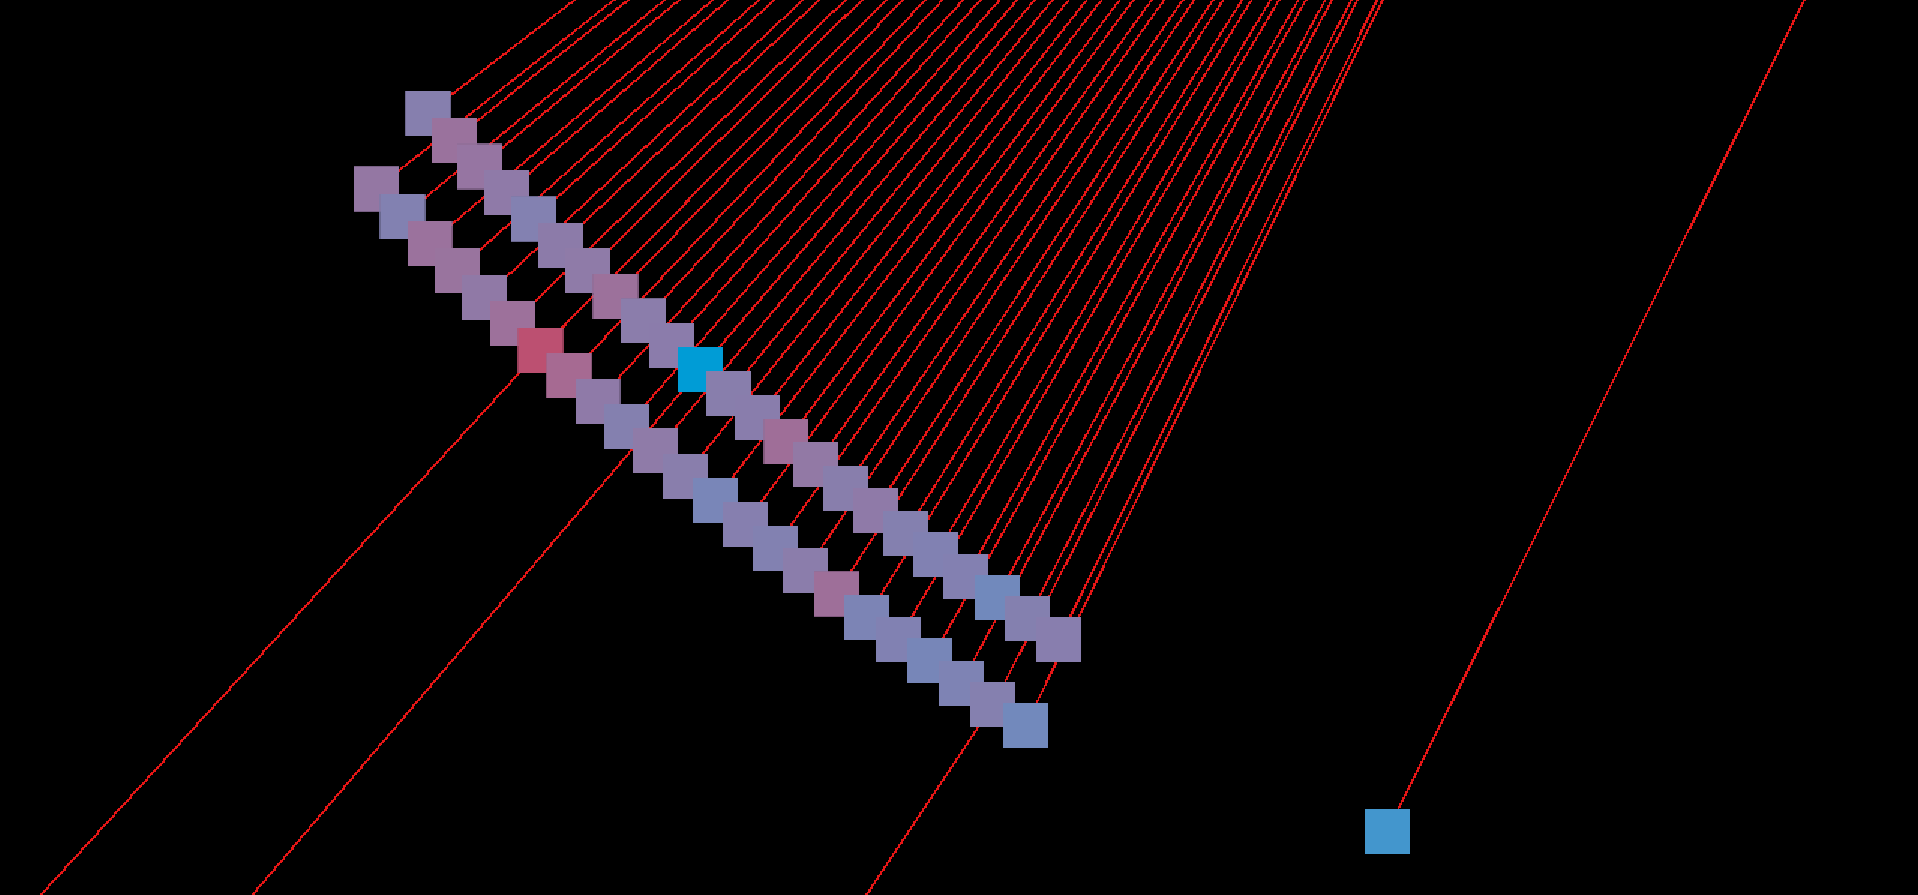
\includegraphics[width=0.45\textwidth]{randomSection.png}
	\caption{This image shows a variety of colors attributed to nodes based on commit frequency of that subsystem.}
	\label{in}
\end{figure}

\subsection{Color Encoding}
\label{colE}
Initially, node colors were determined by a ratio between each subsystems number of commits to the maximum observed number of commits. However, due to a large range in commit data - from 0 to over 500,000 - most nodes appeared as indistinguishable shades of green. The average was somewhere around 1000 commits per subsystem. Except for a select few nodes, the graphs color was monochromatic.

To address this, we implemented a logarithmic transformation to the ratio. This compressed the dynamic range of the nodes. Special cases had to be handled explicitly: $\log(0)$ is undefined and $\log(1)$ returned an unintended blue color - signifying $0$ commits made on the maximally committed node. This logarithmic scaling fixed the issue with most nodes looking identical. Nodes now take on a range of colors from blue (fewer commits) to red (more commits).

 This heat-map approach is useful because it makes it obvious to the user which nodes (or subsystems) have been modified the most. An example of variety in node color can be seen in Figure \ref{in}.



\subsection{Graph Construction}
\label{graphC}
The graph was constructed and rendered using Unity through C\# scripting. Unity was chosen because of its support for real-time user interfaces, and efficient handling of large-scale 2D elements.

Upon startup, the tool reads the preproccessed text file output by the Java parser. This file encodes three pieces of information: (i) the heirarchical parent-child relationships between subsystems, (ii) the total number of commits made to each subsystem, and (iii) the color value computed from the log-scaled heat-map encoding system described in Subsection \ref{colE}.

In Unity, each subsystem is represented as a Node GameObject. Each Node stores the subsystems name, commit amount, associated color, and list of child nodes. Then Edge GameObjects were drawn between Nodes corresponding to each of their child nodes list.

To construct the graph visually, we used a recursive algorithm to iterate through the hierarchy starting from the root node. Thus, creating a radial layout. At each radius from the center, nodes are distributed evenly along an arc around their parent node. This layout helps user's movement along the graph more than a tradition tree layout - such as a binary tree. 

This visualization method was helpful for user movement around the graph, however node crowding becomes an issue in deeper levels. This will be discussed in further detail in Section \ref{futDir}.

\begin{lstlisting}[caption={Recursive portion of radial layout code in C\#}, label={lst:layoutRadial}]
void LayoutRadial(SubsystemLoader.SubsystemNode node, Vector2 center, float radius, float startAngle, float angleRange, int depth, bool placeOnInnerRing)
{

    for (int i = 0; i < node.children.Count; i++)
    {
        float childStartAngle = startAngle + i * angleStep;
        bool childOnInner = (i % 2 == 0);
        LayoutRadial(node.children[i], rootCenter, radius, childStartAngle, angleStep, depth + 1, childOnInner);
    }
}
\end{lstlisting}




\subsection{UI/UX}
Our visualization implementation is interactive. In particular, the user is able to zoom in/out camera allowing examination of broad system structure and individual nodes. The camera can also be panned freely, supporting exploration across the different regions of the graph. These navigational features are necessary considering the size and density of the data. 

To support data inspection, each node is clickable. Clicking on a node reveals the subsystem’s name and its commit count, providing detailed context on demand. An example of the node information panel is shown in Figure \ref{inner}.

This interactive functionality was implemented using Unity's UI Event System and Canvas System, which allows for real-time responses as mentioned in Subsection \ref{graphC}. Nodes were assigned listeners, while camera controls were mapped to the usual bindings. These features allow for in-depth exploration of the Linux subsystem structure.

\begin{figure}[h!]
	\centering
	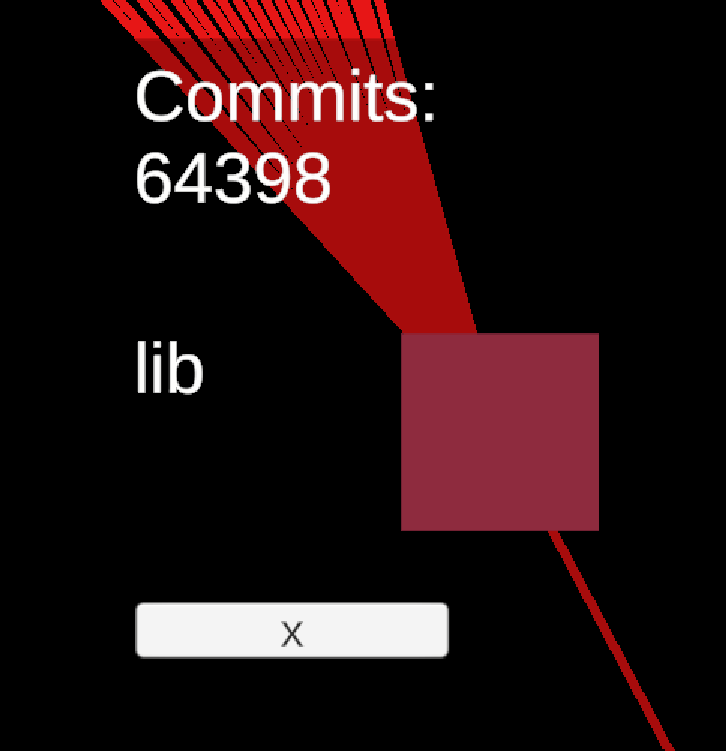
\includegraphics[width = .3\textwidth]{commitPanel.png}
	\caption{View of the tool showing the info panel that appears on click.}
	\label{inner}
\end{figure}






\section{Results and Discussion}
\label{resAndDisc}

Most nodes take on a bluish-purple hue, meaning that most subsystems experience some level of commit activity. We observed that commit density peaked at the third hierarchical level, and gradually decreased as nodes extended further. This suggests that subsystems closer to the core tend to be more actively developed.

 Clusters of high-commit nodes were often located near one another. In particular, when the parent node exhibited a high commit count (appeared red), its child subsystems frequently showed moderate commit activity (appeared purple). This indicated that when a parent subsystem is modified, the children tend to be too. This pattern implies that changes to a parent subsystem cascades into its descendants, showing structural dependencies.

Another thing we noticed was that node density peaked at three levels deep, reinforcing the idea that development is concentrated within mid-level systems. Deeper, more specialized branches were sparser, and received fewer commits. This suppors the idea that niche subsystems are modified less frequently.

\begin{figure}[h!]
	\centering
	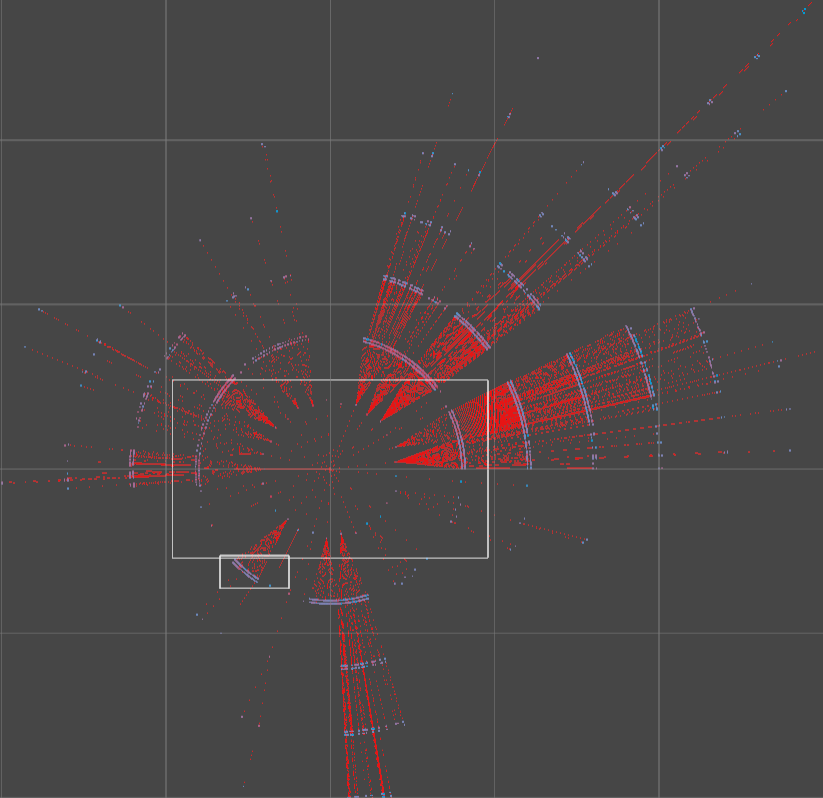
\includegraphics[width=0.4\textwidth]{wholeThingMostly.png}
	\caption{Unity Scene view that shows how large the graph became with only a subsection of Linux commit data. The small rectangle is what is shown in Figure \ref{in}.}
	\label{out}
\end{figure}

This tool can assist developers in understanding how and where the Linux kernel is changing. When organized hierarchically, the tool illuminates intuitive ideas as to why commits are distributed the way they are. This can help contributors identify high-churn areas and under-maintained modules. In doing so, it provides potential applications in software evolution analysis, maintenance prioritization, and onboarding.



\section{Future Directions and Limitations}
\label{futDir}

The current state of the tool fulfills its original purpose of visualizing Linux commit data. However, there are still many ways the tool could be improved to both help with the user experience and usefulness of the tool.

The tool does not keep track of some important data regarding the commits such as the time the commit was made or the author of the commit. These would a great first step in improving the tool. Furthermore, the tool is currently working on a dataset from 2023. A future improvement would be cloning the Linux GitHub repository for commit data rather than relying on the Zenodo dataset \cite{zenodo} we have been using.

Another implementation that would help developers using this tool would be filters to remove redundant or unnecessary information. The ability to sort by what dates the desired commits were made on, by author or by which subsystems the user is interested in would help this tool be more useful for developers. 

These filters would also help with the largest limitation of this tool, which is scalability. We used a small subsection of Linux commit data and yet the graph constructed is enormous. In Figure \ref{out}, it is clear to see that the graph is expansive and for a user to search that for a desired subsystem would be unrealistic. 

A further issue that comes from scalability is node overlap and crowding. For nodes with a large number of children, the arc length's required to space the nodes nicely are too large to be viable. This is because the distance between concentric circles would have to be increased which would make the graph many times larger than it already is.

% talk about node overlap. ok.



\section*{Acknowledgments}
Thank you Belmont University Summer Undergraduate Research Fellowships in the Sciences (SURFS) program and God.




\bibliographystyle{IEEEtranS}
\bibliography{mybib}

\vspace{12pt}


\end{document}